\documentclass{article}
\usepackage{microtype}
\usepackage{graphicx}
\usepackage{subfigure}
\usepackage{booktabs}
\usepackage{multirow}
\usepackage{hyperref}
\newcommand{\theHalgorithm}{\arabic{algorithm}}
\usepackage[accepted]{icml2021}
\usepackage[T1]{fontenc}
\hypersetup{hypertexnames=false}
\makeatletter\let\tableinput\@@input\makeatother
\makeatletter
\patchcmd{\printAffiliationsAndNotice}{Correspondence to: \icmlcorrespondingauthor@text.}{}{}{}
\renewcommand{\Notice@String}{Interim course project report. Not a conference publication.}
\makeatother
\icmltitlerunning{Explicit hand-shape features for ASL recognition}
\begin{document}
\twocolumn[
\icmltitle{Interpretable Hand-Shape Features for ASL Letter Recognition\\Do Explicit Descriptions Add Value Beyond Geometric Descriptors?}
\begin{icmlauthorlist}
\icmlauthor{Author details to be added}{ou}
\end{icmlauthorlist}
\icmlaffiliation{ou}{Open Universiteit}
\icmlcorrespondingauthor{}{}
\icmlkeywords{ASL, fingerspelling, feature engineering, joint angles, ablation}
\vskip 0.3in
]
\printAffiliationsAndNotice{}
\begin{abstract}
Can descriptions such as bent, extended, spread or touching improve a letter recognizer that already receives hand geometry? Webcam confusions motivated a comparison of categorical hand features, workbook agreement scores and continuous joint measurements added to a Shin-based reference. SVM and LightGBM used the same 60,251 accepted Kaggle ASL Alphabet images and five grouped validation folds. The full feature package did not improve SVM accuracy (97.628\% versus 97.637\%). Adding joint measurements from estimated world landmarks reached 97.748\% and 0.97524 macro-F1: 143 errors corrected, 76 correct predictions lost, net +67. A control deriving joint measurements from the same coordinates as Shin reached only 97.643\%, net +4; replacing directions with those measurements reduced accuracy to 94.511\%. Explicit descriptions therefore do not reliably improve this geometric reference, and the small world-coordinate gain cannot be attributed to the bending-angle formula alone. These exploratory results concern representation, not new sensing information or demonstrated reliability on unseen people and webcam conditions.
\end{abstract}

\section{Brief Introduction}
American Sign Language (ASL) fingerspelling recognition can be approached by locating hand landmarks and classifying their arrangement. This project concerns individual letter images, rather than continuous signing or the movement required for letters such as J and Z. Its practical motivation came from a webcam recognizer: I could intend the same letter but receive a different prediction after changing my hand position. I noticed C/D/O and U/V/R confusions. Those observations were informal and motivated questions; they did not measure error rates.

The recognizer followed the geometric approach of \citet{shin2021}. Instead of learning directly from image pixels, it describes distances and directions between hand points. This prompted an intuitive question: could explicit descriptions such as ``the middle finger is bent'', ``these fingers cross'' or ``the thumb touches the index finger'' make the distinction easier?

I developed a workbook of expected hand features and a tool to inspect the measured hand. Continuous joint measurements serve as a comparison with the broader categorical descriptions. A later control uses the same coordinates as Shin to distinguish representation from coordinate source. Figure~\ref{fig:core-process} summarizes the investigation. The contribution is a matched empirical comparison, including negative results; no new classification algorithm or independent sensor information is claimed.

The main research question is: \emph{Do interpretable hand-shape descriptions add value to a Shin-based ASL letter recognizer?} Three questions make it testable:
\begin{enumerate}
\item Does the full package of categories, workbook scores and joint measurements improve the reference, and does classifier choice matter?
\item Do continuous measurements help, and does their coordinate representation matter?
\item Which letters benefit or regress, and how consistent are the observed differences?
\end{enumerate}
The following sections connect these questions to prior work, explain the comparisons, report their outcomes and discuss their limits. Later webcam and augmentation experiments are supporting diagnostics, not additional requirements for answering the main question. Technical details and complete results are in the separate appendix.

\begin{figure*}[t]
\centering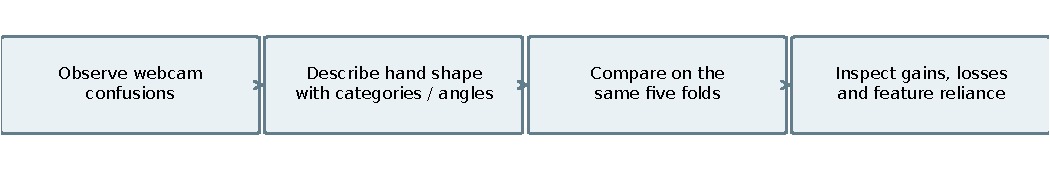
\includegraphics[width=\linewidth]{figures/core_pipeline.pdf}
\caption{The research sequence. Webcam observations motivated feature design; the primary evidence comes from matched dataset comparisons and analysis of both improvements and regressions.}
\label{fig:core-process}
\end{figure*}

\section{Related Works}
\citet{shin2021} represent hand landmarks through pairwise distances and directions and compare SVM with LightGBM. Their approach provides the reference representation here. This study asks whether more explicit hand descriptions help when that geometric information is already present. Additional features may reorganize existing information rather than supply independent evidence.

MediaPipe Hands estimates a hand skeleton from an RGB image \citep{zhang2020}. The classifier therefore receives measurements produced by another model. Describing a feature in meaningful terms does not guarantee that the landmark estimate measures it accurately. In contrast, the colour-and-depth approach of \citet{pugeault2011} uses additional sensing information. The present work retains ordinary RGB input and investigates representations of its estimated landmarks.

LightGBM learns boosted decision trees \citep{ke2017}. Its split-based decisions provide a plausible alternative for mixed hand measurements, while an RBF SVM separates examples through similarity in feature space. Comparing both tests whether a feature package's usefulness depends on the learner. The tested fixed profiles do not establish which algorithm would win after equally extensive optimization.

Interpretability also needs care. \citet{fisher2019} show that variable importance depends on the fitted model. Accordingly, this study distinguishes shuffling a feature group to test model reliance from removing it and retraining to test added value. Finally, repeatedly selecting models using the same evaluation can produce optimism \citep{cawley2010}. The experiments below are therefore reported as exploratory comparisons, with their scope separated from final-test claims.

\section{Methods}
\subsection{From Observations to Representations}
The reference contains 820 Shin-style measurements: 190 normalized distances and 630 directions relative to the image axes. These are not explicit joint-bending angles, but the directions of adjacent segments already determine their interior angle. The hypothesis is that a different representation helps learning, not that Shin lacks hand-shape information. I used three additions:
\begin{itemize}
\item \textbf{Categories:} 70 one-hot inputs describe bending, spread, suspected crossing, thumb shape and contact, including unknown states.
\item \textbf{Workbook scores:} 26 inputs measure agreement with the expected features of each candidate letter. Slash-separated workbook values are allowed alternatives. Every candidate score is computed without reading the image's true label.
\item \textbf{Joint measurements:} 14 internal angles and a signed thumb-MCP deviation, giving 15 continuous inputs. MCP measurements are landmark-based proxies rather than clinical joint measurements.
\end{itemize}
A straight internal angle approaches $180^\circ$; bending reduces it. Categories compress measurements into labels, while continuous values retain finer variation. The original additions use estimated world landmarks, whereas Shin uses normalized image landmarks. A control recomputes the 15 measurements from Shin's exact coordinates: adding them gives 835 inputs; replacing the 630 directions gives 205 (190 distances + 15 measurements). No images are redetected. Most comparisons retain all reference inputs; the replacement control is explicitly separate.

\subsection{Models and Checks}
The main learner is an RBF SVM with $C=10$, \texttt{gamma=scale} and balanced classes. It balances separation against classification errors. LightGBM uses 100 trees, 31 leaves, learning rate 0.1 and minimum child size 20. We retain these project profiles across representation comparisons. Median imputation and standardization of angle inputs are learned only from the fitting partition. Baseline measurements and categorical/workbook inputs pass through unchanged. The appendix gives the objectives, formulas and exact schemas.

To investigate contribution, I removed feature groups and retrained, and separately shuffled groups in held-out inputs of a fitted full-package model. Shuffling used five repeats and up to 100 images per letter per fold. Correlated features can compensate for one another, so these reliance measures are neither causal effects nor additive percentages of importance.

Bounded weighting checks used five outer and three inner group folds, with inner samples capped at 150 images per letter. They do not remove selection effects from the wider exploratory sequence. Settings and detailed checks are in the appendix.

\section{Experimental Results}
\subsection{Dataset and Evaluation}
Kaggle ASL Alphabet supplies 78,000 training images, 3,000 for each A--Z label. Only 60,251 images with exactly one accepted hand detection enter the comparisons: 77.25\% coverage. Consequently, classification scores are conditional on successful landmark extraction. The small supplied test set duplicates training images and was excluded. Historical landmark records do not retain the confidence thresholds; the intended default extraction settings cannot be independently confirmed.

Every main comparison uses the same accepted images and frozen five group folds. Adjacent image numbers are grouped into six filename blocks, distributed across the folds. Each image receives one prediction from a model that was not fitted on it. These groups are not verified people; possible similarity across blocks limits claims about new signers. Accuracy is pooled over all held-out predictions. Macro-F1 averages the 26 letter F1-scores, giving equal weight to each letter and accounting for false positives as well as missed examples. No untouched final classification test is available.

\subsection{RQ1: Does the Broader Feature Package Help?}
Table~\ref{tab:core-results} gives the matched results. For SVM, all 111 additions together reach 97.628\% accuracy, slightly below the 97.637\% reference. LightGBM improves from 97.097\% to 97.164\% with that package, but remains below the tested SVM configurations. Thus the package's effect depends on the learner, and it does not consistently improve the reference.

\begin{table*}[t]
\centering\caption{Pooled five-fold results on 60,251 accepted images. Every row retains the 820 reference inputs. ``All additions'' adds 70 categories, 26 workbook scores and 15 world-joint measurements. The final row instead derives joints from Shin's coordinates. These are exploratory results, not independent final-test scores.}
\label{tab:core-results}
\begin{tabular}{lrrrrr}\toprule
 & & \multicolumn{2}{c}{SVM} & \multicolumn{2}{c}{LightGBM}\\
Representation & Inputs & Accuracy (\%) & Macro-F1 & Accuracy (\%) & Macro-F1\\\midrule
\tableinput core_results.tex
\bottomrule\end{tabular}
\end{table*}

Feature removal clarifies the SVM result. Removing the 70 categories from the full package improves accuracy to 97.744\%, the angles-plus-workbook row. Removing angles instead leaves categories and workbook scores and reaches 97.593\%. These comparisons support the continuous representation in this setting. They do not isolate categories alone without workbook scores, or prove that categorical descriptions are inherently unhelpful.

\subsection{RQ2: Do Joint Measurements Add Value?}
Adding the 15 world-joint measurements to the reference reaches 97.748\% SVM accuracy and 0.97524 macro-F1, versus 97.637\% and 0.97386. Workbook scores add no further benefit. For LightGBM, the world-joint addition reduces accuracy to 97.017\%. This is a small, learner-specific result.

The coordinate control qualifies its interpretation. Adding same-coordinate joint measurements reaches 97.643\% and 0.97403 macro-F1 for SVM: 89 errors corrected and 85 correct predictions lost, net +4, not +67. LightGBM loses 34 correct predictions. Replacing directions with distances plus same-coordinate joints lowers accuracy to 94.511\% (SVM) and 93.942\% (LightGBM). The full control is in Appendix~K. It gives no convincing overall benefit from making bending explicit in Shin's coordinates; the earlier world-coordinate gain cannot be attributed to the angle formula alone.

Grouped permutation gives complementary evidence. In the full-package SVM, shuffling joint measurements reduces macro-F1 by an average 0.570 percentage points, versus 0.049 for categories and 0.008 for workbook scores. This indicates greater reliance on the angles in that fitted model; it is not the amount by which adding them improves the reference. The removal and matched-addition results are needed for that claim. Broad feature weighting did not yield a convincing additional overall benefit under the bounded search.

\subsection{RQ3: Who Benefits, and How Stable Are Differences?}
The world-joint addition fixes 143 formerly incorrect images and loses 76 formerly correct ones: net +67 out of 60,251, or 0.1112 percentage points. It improves all five outer folds and six filename blocks, but the gain is small. A block-resampling sensitivity range of 0.0374--0.1947 percentage points is descriptive, not an independent-test confidence interval or significance result (Appendix~D). The same-coordinate addition instead improves three folds and worsens two (Appendix~K).

\begin{figure*}[t]
\centering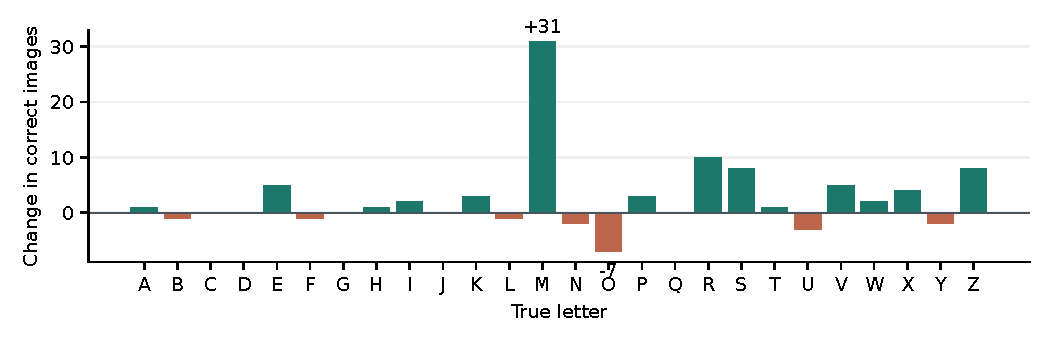
\includegraphics[width=\linewidth]{figures/core_letter_effects.pdf}
\caption{Change in correct true-letter images after adding world-joint measurements to the SVM reference. Green bars show gains and orange bars losses, summing to +67. This is the earlier world-coordinate comparison, not the same-coordinate control (+4). Full letter metrics and confusion matrices are in Appendices~A--B.}
\label{fig:letter-effects}
\end{figure*}

Figure~\ref{fig:letter-effects} and Table~\ref{tab:core-letters} show why the pooled gain needs qualification. M gains 31 correct images, while O loses seven. N loses two true-letter recoveries yet improves in F1, because false-positive behaviour also changes. Different metrics therefore answer different questions. The angle model still has 142 R$\rightarrow$U, 141 N$\rightarrow$M, 102 M$\rightarrow$N and 41 D$\rightarrow$O errors. These residual patterns matter more than selecting only favourable letters.

\begin{table}[t]
\centering\caption{Selected letter effects; F1 is a percentage and $\Delta n$ is the change in correctly recovered true-letter images. The appendix includes every letter.}
\label{tab:core-letters}
\begin{tabular}{lrrrr}\toprule
Letter & Images & Base F1 & World F1 & $\Delta n$\\\midrule
\tableinput core_letter_rows.tex
\bottomrule\end{tabular}
\end{table}

Targeted index-joint weighting did not yield a convincing overall benefit; selected weights varied across folds (Appendix~D).

\subsection{Supporting Webcam Diagnostics}
A later guided development round retained all 27 planned C/D/O attempts with predictions hidden. The reference and angle models each recognized 17/27. Small tilt augmentation recognized 18/27; C-only tilt did not improve the predictions. Later 2D-angle and G/H-specific investigations likewise did not establish a general solution. Those results are retained in Appendix~I--J, outside the primary feature comparison.

These observations illustrate a limit, not a new webcam accuracy claim. For example, one selected G had middle-PIP flexion consistent with training G but was still H; another H with visible palm was G. Palm/back viewpoint, other measurements and learned decision boundaries may all contribute. Selected errors cannot establish the frequency or main cause of failure, and projected image angles do not prove that an estimated 3D angle is wrong.

\clearpage
\section{Discussion}
The interpretable feature package does not consistently improve the geometric reference. Its SVM result is slightly worse; the positive world-joint result is small and does not reproduce as a meaningful gain with same-coordinate joints. The evidence supports a bounded comparison of representations, not a general performance improvement.

Joint angles and categories largely re-express landmark geometry; categorical flexion also derives from thresholded angles. The control therefore addresses redundancy directly. Coordinate estimates, scaling and model geometry may contribute to the different outcomes; their individual effects are not isolated. Removing direction features also discards axis-relative orientation, which may distinguish letters. Poor replacement performance does not prove that joint calculations are wrong or that categories are intrinsically unhelpful.

Several limitations bound the answer. The workbook and its relaxations were developed exploratorily, not nested inside all later evaluations. Multiple representations were inspected on the same folds, despite nested tuning within particular searches. The strongest observed result should therefore not be treated as an unbiased estimate of a selected final system. Fixed classifier profiles also limit conclusions about algorithm superiority. Filename-block grouping cannot establish signer-independent performance, and detection filtering excludes difficult images before classification.

The source article reports 87.60\% ASL Alphabet accuracy, not a matching F1 score. Our filtering, split and training settings differ, so the local 97\% scores are neither an exact reproduction nor evidence of outperforming that article. Live examples further show that a strong conditional dataset score does not guarantee reliable use under different capture conditions. No evidence here establishes that back-of-hand views are systematically worse, or that the early U/V/R observations have been solved.

The report and much of the software were AI-generated. AI-assisted code inspection, unit tests and reconciliation with stored predictions were used in an attempt to verify the implementation. These checks do not constitute independent human code review, linguistic review of the workbook or validation of estimated anatomy. The author should verify the interpretation and references before submission. Participants should consent to webcam collection; saved images remain local by default. Single-frame letter recognition should not be presented as full sign-language understanding or a replacement for qualified interpretation.

\section{Conclusions}
Interpretable hand descriptions give no consistent advantage over the Shin-based reference in this evaluation. The full package does not improve SVM accuracy. World-joint additions yield a small net gain of 67 images; same-coordinate additions yield only four, and replacing directions loses 1,883. The world result is specific to its representation and learner, with letter-level regressions and no independent final-test confirmation.

The contribution is testing whether meaningful descriptions add predictive value when geometry is already available, and documenting their limits through matched comparisons and error analysis. Further G/H rotation experiments should separate feature-space rotation from rotating images and rerunning detection, and use a predefined, signer/session-separated evaluation. Current dataset scores do not establish webcam robustness.

\clearpage
\bibliography{references}
\bibliographystyle{icml2021}
\end{document}
